\chapter{Optimizing Calibration Efficiency} \label{chap:Time}

\noindent This chapter explores strategies to reduce the calibration time of the algorithm. The initial approach involved transcribing the algorithm from Python to C++ to leverage the latter’s greater computational efficiency. However, despite the significant development effort required, this optimization yielded only a marginal improvement, reducing calibration time by approximately 1\%.

\noindent Given the limited success of this approach, an alternative solution was pursued. It was identified that the primary bottleneck in the program was the process of saving snapshots to the computer’s disk during each iteration, which significantly slowed down execution. To address this, a virtual graphics card provided by wTVision was utilized, enabling direct communication with Python and allowing snapshots to be transferred in real-time instead of being stored on disk. This modification substantially improved the calibration efficiency.

\section{MockBoard} \label{sec:MockBoard}   

\noindent The MockBoard is a virtual graphics card provided by wTVision that allows for the real-time transfer of images to the computer. This eliminates the need to save snapshots to disk, which significantly 
reduces the time required for calibration. The MockBoard is a software solution that emulates a video capture card, enabling the computer to receive video input directly from the $R^3$ software. This allows the computer to process the 
iamges in real-time, without the need to save snapshots to disk. The MockBoard is a proprietary software solution developed by wTVision, and is not available to the general public. 

\noindent To use Mockboard in the calibration algorithm, the following steps are required:

\begin{enumerate}
    \item Open the $R^3$ software in administrator mode.
    \item Select MockBoard as the output in the $R^3$ software, like in figure \ref{fig:MockBoard}.
\end{enumerate}

\begin{figure}[h]
    \centering
    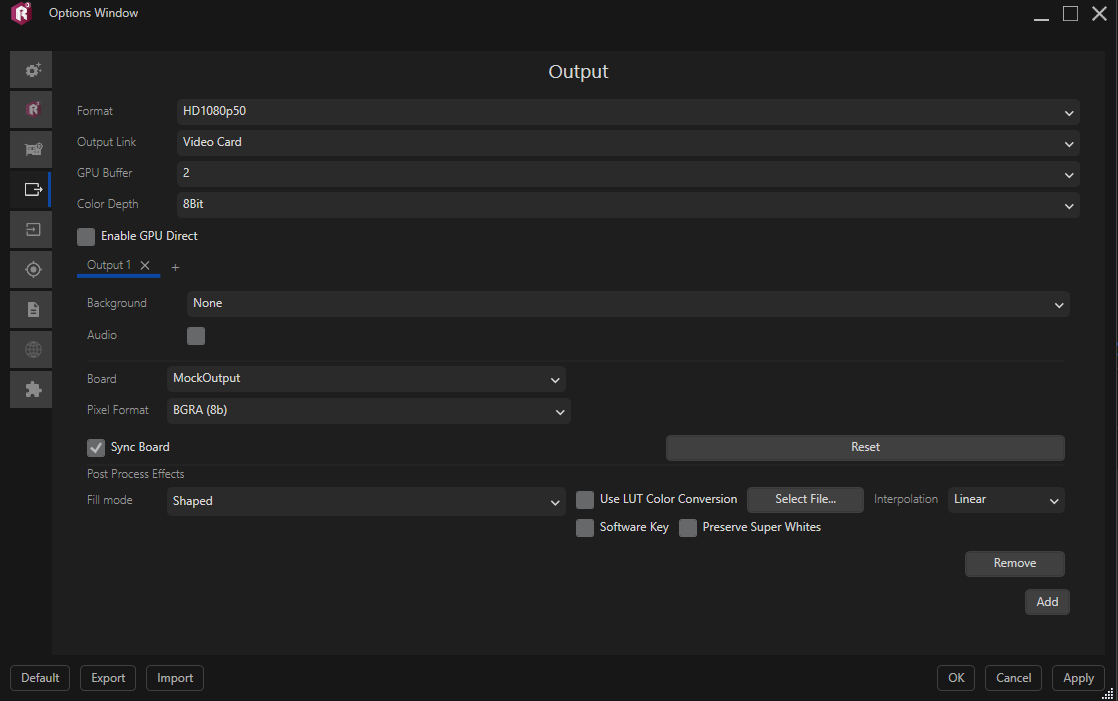
\includegraphics[width=\textwidth]{Images/05optimize/Mockboard.png}
    \caption{Selecting MockBoard as the output in the $R^3$ software.}
    \label{fig:MockBoard}
\end{figure}

\subsection{Communication with MockBoard} \label{subsec:MockBoardComm}

\noindent The MockBoard functions as a local webapi with the following url:

"http://localhost:1987/apiv1/MockCard/MockOutput/GetImage"

\noindent Figure \ref{fig:webapi} illustrates its corresponding web page. 

\begin{figure}[h]
    \centering
    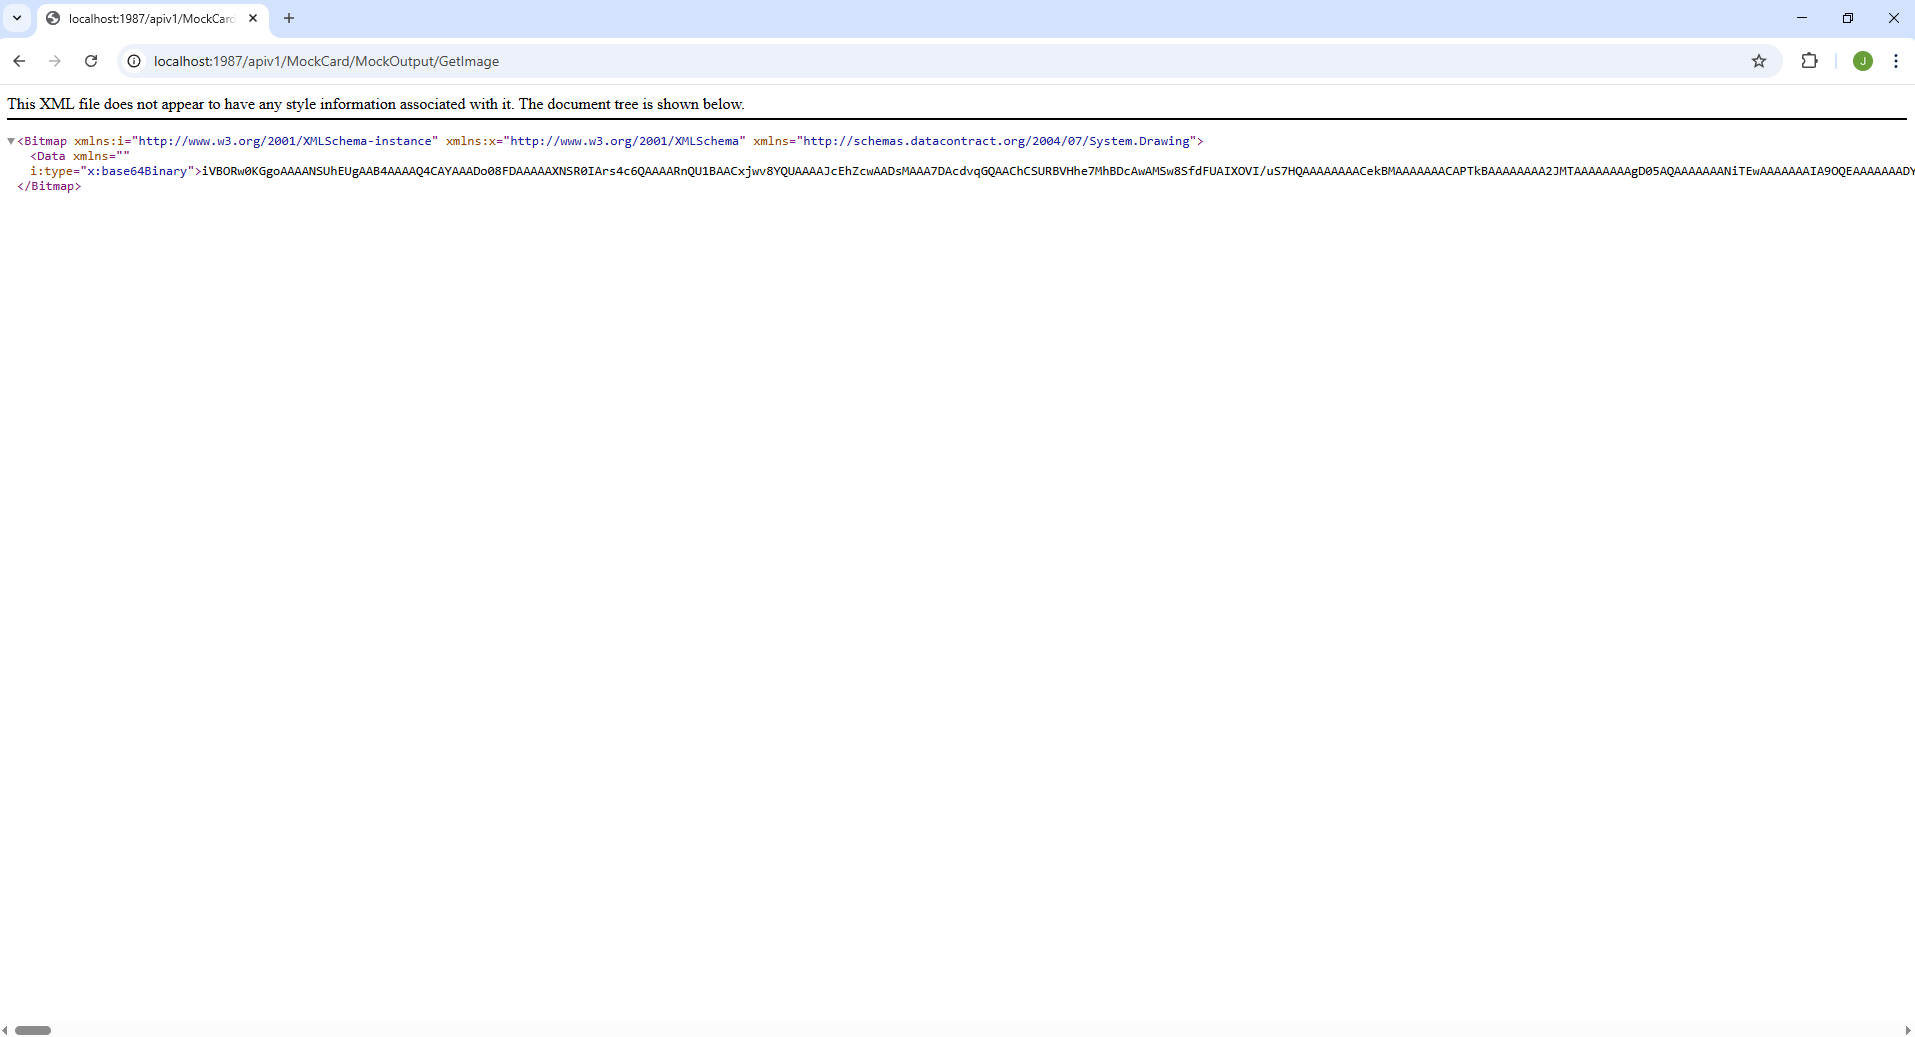
\includegraphics[width=\textwidth]{Images/05optimize/webapi.png}
    \caption{MockBoard web page.}
    \label{fig:webapi}
\end{figure}

\noindent As demonstrated in figure \ref{fig:webapi}, this url returns a string of an image in base64 format.
To communicate with it using Python, http requests are used in order to return this string. The following steps outline how to estaplish communcation between the 
Python script and the MockBoard:


\begin{enumerate}
    \item First, the correct headers need to be added. This can be achieved by using the following code:
    
    \begin{verbatim}
    response = requests.get(url, headers=headers)
    \end{verbatim}
    
    These headers are displayed in Table~\ref{tab:headers} in the annex chapter~\ref{chap:annex}.

    \item Using HTTP requests it is possible to obtain the image in base64 format.
    \item The base64 image is then converted into a png image using the base64 and BytesIO Python libraries.
\end{enumerate}


Using the MockBoard, it takes exacly 0.015 seconds to obtain an image, which is a significant improvement over the previous method of saving snapshots to disk, which took around 0.3 seconds. This 
improvement should reduce the algorithm's calibration time by at least 90\%.

\section{Results} \label{sec:Results}

\noindent The calibration algorithm was tested using the MockBoard to evaluate the impact on calibration time. The results are presented in figure \ref{fig:results}.

\begin{figure}[ht]
    \centering
    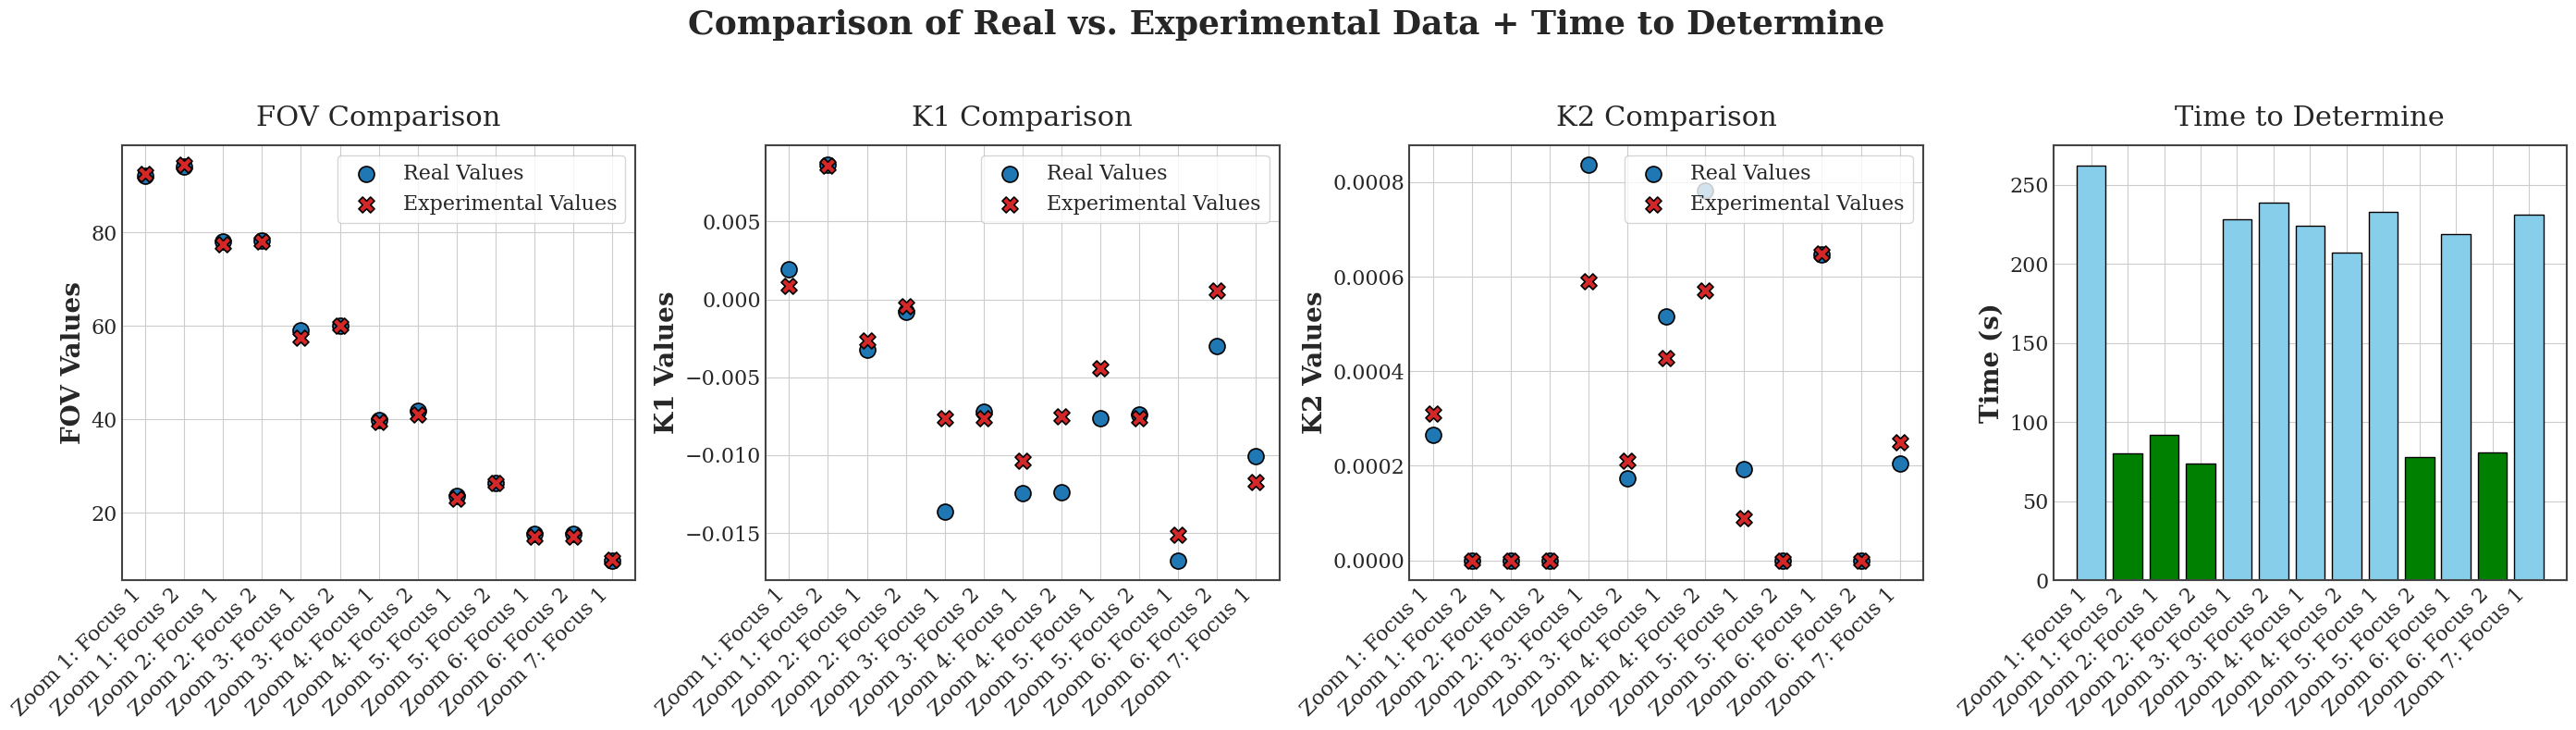
\includegraphics[width=\textwidth]{Images/05optimize/r_graph.png}
    \caption{Distortion calibration results using the MockBoard.}
    \label{fig:results}
\end{figure}

\noindent As shown in figure \ref{fig:results}, the calibration time was significantly reduced, only taking 35.1 minutes to calibrate 13 levels of zoom/focus, 
using the old method would've taken above 120 minutes. This significant improvement in efficiency demonstrates the potential 
of the MockBoard to optimize the calibration algorithm.

\noindent As expected, when K2 is 0 it takes less time to calibrate. The green bars in figure \ref{fig:results} represent the time taken to calibrate when K2 is 0, while the blue bars represent the 
time taken to calibrate when K2 is not 0.